%% \documentclass[archE, portrait, fontscale=0.32]{baposter} % "Arch E" is the correct size for a 36"x48" poster
\documentclass[ansiepaper, portrait, fontscale=0.35]{baposter} % "ANSI E" is the correct size for a 34"x44" poster
%% \documentclass[a0paper, portrait, fontscale=0.34, margin=1.5cm]{baposter} % 
%% \documentclass[eshg, portrait, fontscale=0.29]{baposter} % 
\usepackage{times}
\usepackage{calc}
\usepackage{graphicx}
\usepackage{amsmath}
\usepackage{amssymb}
\usepackage{relsize} % For \smaller
\usepackage{multirow}
\usepackage{multicol}
\usepackage{longtable}
\usepackage{bm}
\usepackage{graphicx}
\usepackage{palatino}
\usepackage{url}
\selectcolormodel{RGB}

%%%%%%%%%%%%%%%%%%%%%%%%%%%%%%%%%%%%%%%%%%%%%%%%%%%%%%%%%%%%%%%%%%%%%%%%%%%%%%%%
%%%% Some math symbols used in the text
%%%%%%%%%%%%%%%%%%%%%%%%%%%%%%%%%%%%%%%%%%%%%%%%%%%%%%%%%%%%%%%%%%%%%%%%%%%%%%%%
% Format 
\newcommand{\Matrix}[1]{\begin{bmatrix} #1 \end{bmatrix}}
\newcommand{\Vector}[1]{\Matrix{#1}}
\newcommand*{\SET}[1]  {\ensuremath{\mathcal{#1}}}
\newcommand*{\MAT}[1]  {\ensuremath{\mathbf{#1}}}
\newcommand*{\VEC}[1]  {\ensuremath{\bm{#1}}}
\newcommand*{\CONST}[1]{\ensuremath{\mathit{#1}}}
\newcommand*{\norm}[1]{\mathopen\| #1 \mathclose\|}% use instead of $\|x\|$
\newcommand*{\abs}[1]{\mathopen| #1 \mathclose|}% use instead of $\|x\|$
\newcommand*{\absLR}[1]{\left| #1 \right|}% use instead of $\|x\|$

\def\norm#1{\mathopen\| #1 \mathclose\|}% use instead of $\|x\|$
\newcommand{\normLR}[1]{\left\| #1 \right\|}% use instead of $\|x\|$
\newcommand*{\p}[1]{\Pr{\left\{ #1\right\}}}  % Probability

%%% Global Settings %%%%%%%%%%%%%%%%%%%%%%%%%%%%%%%%%%%%%%%%%%%%%%%%%%%%%%%%%%%

\graphicspath{{fig/}}	% Root directory of the pictures 
\tracingstats=2			% Enabled LaTeX logging with conditionals

\definecolor{bordercol}{RGB}{40,40,40}
\definecolor{Yellow}{RGB}{253,176,61}
\definecolor{OxfordBlue}{RGB}{0,0,102}
\definecolor{TodaiBlue}{RGB}{90,141,201}
\definecolor{BaylorBlue}{RGB}{0,62,126} % #003E7E
\definecolor{BaylorBurgundy}{RGB}{98, 27, 75}
\definecolor{LighterBlue}{RGB}{241,244,255}
% A coloured circle useful as a bullet with an adjustably strong filling
\newcommand{\cir}[1]{%
\tikz{\useasboundingbox (-0.2em,-0.32em) rectangle(0.2em,0.32em); \draw[draw=BaylorBurgundy,fill=BaylorBurgundy!#1!white,line width=0.03em] (0,0) circle(0.2em);}}
\newcommand{\captionfont}{\footnotesize}
\newcommand{\tri}{\color{BaylorBurgundy}{$\triangleright$}}
\newcommand{\hf}[1]{{\color{BaylorBurgundy}\textbf{#1}}}
%%%%%%%%%%%%%%%%%%%%%%%%%%%%%%%%%%%%%%%%%%%%%%%%%%%%%%%%%%%%%%%%%%%%%%%%%%%%%%%%
% Multicol Settings
%%%%%%%%%%%%%%%%%%%%%%%%%%%%%%%%%%%%%%%%%%%%%%%%%%%%%%%%%%%%%%%%%%%%%%%%%%%%%%%%
\setlength{\columnsep}{0.7em}
\setlength{\columnseprule}{0mm}


%%%%%%%%%%%%%%%%%%%%%%%%%%%%%%%%%%%%%%%%%%%%%%%%%%%%%%%%%%%%%%%%%%%%%%%%%%%%%%%%
% Save space in lists. Use this after the opening of the list
%%%%%%%%%%%%%%%%%%%%%%%%%%%%%%%%%%%%%%%%%%%%%%%%%%%%%%%%%%%%%%%%%%%%%%%%%%%%%%%%
\newcommand{\clist}[1]{%
\begin{list}{\labelitemi}{\leftmargin=1em}
\setlength{\parindent}{5em}
\setlength{\itemsep}{0.2em}
\setlength{\parskip}{0em}
\setlength{\parsep}{0em}
#1
\end{list}
}

%% Define a new 'leo' style for the package that will use a smaller font.
\makeatletter
\def\url@leostyle{%
  \@ifundefined{selectfont}{\def\UrlFont{\sf}}{\def\UrlFont{\small\color{BaylorBlue}\rmfamily}}}
\makeatother
%% Now actually use the newly defined style.
\urlstyle{leo}
%%%%%%%%%%%%%%%%%%%%%%%%%%%%%%%%%%%%%%%%%%%%%%%%%%%%%%%%%%%%%%%%%%%%%%%%%%%%%%
%%% Begin of Document
%%%%%%%%%%%%%%%%%%%%%%%%%%%%%%%%%%%%%%%%%%%%%%%%%%%%%%%%%%%%%%%%%%%%%%%%%%%%%%

\begin{document}

%%%%%%%%%%%%%%%%%%%%%%%%%%%%%%%%%%%%%%%%%%%%%%%%%%%%%%%%%%%%%%%%%%%%%%%%%%%%%%
%%% Here starts the poster
%%%---------------------------------------------------------------------------
%%% Format it to your taste with the options
%%%%%%%%%%%%%%%%%%%%%%%%%%%%%%%%%%%%%%%%%%%%%%%%%%%%%%%%%%%%%%%%%%%%%%%%%%%%%%
\typeout{Poster rendering started}
%%% Setting Background Image %%%%%%%%%%%%%%%%%%%%%%%%%%%%%%%%%%%%%%%%%%%%%%%%%%
%\background{
%  \begin{tikzpicture}[remember picture,overlay]%
%    \draw (current page.north west)+(-2em,-0em) node[anchor=north west] 
%   {\hspace{-2em}\includegraphics[height=1.1\textheight]{silhouettes_background}};
%  \end{tikzpicture}%
%}


\begin{poster} {
    grid=false,
    % Option is left on true though the eyecatcher is not used. The reason is
      % that we have a bit nicer looking title and author formatting in the headercol
      % this way
    eyecatcher=false, 
    colspacing=0.33cm,               % column spacing
    bgColorOne=white,                % top background color (only color for background=plain)
    bgColorTwo=LighterBlue,          % bottom background color (for background=shadetb)
    %% background=shadetb,
    background=plain,
    borderColor=white!95!BaylorBlue,
    headerColorOne=TodaiBlue,        % top color of inset header gradient
    headerColorTwo=BaylorBlue,       % bottom color of inset header gradient
    headerFontColor=white,
    % Only simple background color used, no shading, so boxColorTwo isn't necessary
    boxColorOne=LighterBlue,
    boxshade=plain,
    headershape=rounded,
    headershade=shadetb,
    headerfont=\Large \bf,
    %% textborder=triangles,
    textborder=faded,
    headerborder=open,
    linewidth=1.2pt
}

    {\sf \Huge
    \vspace{0.6cm}
    \textbf{Collapsed haplotype pattern method for linkage analysis \\ of next-generation sequencing data}
    }
    {
    \begin{minipage}{24.5cm}
      \vspace{0.5cm}
      \sf
      Gao T. Wang, Di Zhang, Biao Li, Hang Dai and Suzanne M.~Leal$^\dagger$ \\

      \vspace{-0.5cm}
      \small
      $^\dagger${Center for Statistical Genetics, Department of Molecular and Human Genetics, Baylor College of Medicine, Houston, Texas, USA} \\
    \end{minipage}
    \begin{minipage}{2cm}
      \vspace{-0.5cm}
      \hspace{0.2cm}
      
\includegraphics[height=2.2cm]{qrcode}
    \end{minipage}
    \begin{minipage}{1cm}
      \vspace{-0.2cm}
      
\includegraphics[height=2cm]{bcm}
    \end{minipage}
    }

%%%%%%%%%%%%%%%%%%%%%%%%%%%%%%%%%%%%%%%%%%%%%%%%%%%%%%%%%%%%%%%%%%%%%%%%%%%%%%
%%% Now define the boxes that make up the poster
%%%---------------------------------------------------------------------------
%%% Each box has a name and can be placed absolutely or relatively.
%%% The only inconvenience is that you can only specify a relative position 
%%% towards an already declared box. So if you have a box attached to the 
%%% bottom, one to the top and a third one which should be in between, you 
%%% have to specify the top and bottom boxes before you specify the middle 
%%% box.
%%%%%%%%%%%%%%%%%%%%%%%%%%%%%%%%%%%%%%%%%%%%%%%%%%%%%%%%%%%%%%%%%%%%%%%%%%%%%%
%%%%%%%%%%%%%%%%%%%%%%%%%%%%%%%%%%%%%%%%%%%%%%%%%%%%%%%%%%%%%%%%%%%%%%%%%%%%%%
  \headerbox{Motivation}{name=intro,column=0,row=0} {
%%%%%%%%%%%%%%%%%%%%%%%%%%%%%%%%%%%%%%%%%%%%%%%%%%%%%%%%%%%%%%%%%%%%%%%%%%%%%%
      \clist{
        \item[\cir{100}] Variant filtering using next-generation sequencing (NGS) data of families has successfully identified many causal mutations for Mendelian diseases, yet such approach 
        \clist{ 
          \item[\tri] May result in many variants to follow-up
          \item[\tri] Is sensitive to mis-classification
            \clist{
              \item[\tri] Sample swaps, phenocopies, reduced penetrance
              }
          \item[\tri] Do not provide statistical evidences
        }
        \item[\cir{100}] Linkage analysis has been a powerful approach to map Mendelian disease loci using genetic marker data, but is under-powered when applied to sequence data, mainly due to lack of heterogeneity in single-nucleotide variants
        \item[\cir{100}] We developed a \hf{\textit{Collapsed Haplotype Pattern}} (CHP) method and a \hf{SEQLinkage} software to utilize NGS data of multiple families for powerful linkage analysis
      }
  }

%%%%%%%%%%%%%%%%%%%%%%%%%%%%%%%%%%%%%%%%%%%%%%%%%%%%%%%%%%%%%%%%%%%%%%%%%%%%%%
  \headerbox{The CHP Method}{name=stats,column=0,below=intro}{
%%%%%%%%%%%%%%%%%%%%%%%%%%%%%%%%%%%%%%%%%%%%%%%%%%%%%%%%%%%%%%%%%%%%%%%%%%%%%%
   Inspired by rare variant ``burden test'' for association, the CHP method tests for linkage with a genetic region rather than with individual variants
    \clist{
        \item[\cir{100}] \hf{Regional markers} are generated for given genomic units
             \clist{
              \item[\tri] \textit{e.g.} genes for exome sequence data
              }
        \item[\cir{100}] CHP regional markers are \hf{more heterozygous}
             \clist{
              \item[\tri] More informative than single variants in tracking the transmission of disease mutations within families, and when analyzing multiple pedigrees in the presence of allelic heterogeneity
              }
          
        \item[\cir{100}] \hf{Tolerates missing data} on causal variant sites
        \item[\cir{100}] No LD pruning required, all variants in data are used
    }
    \textbf{\textit{Complete Collapsing}} 
    \begin{center}
      \begin{tabular}{c}
        \hspace{1em}\scalebox{0.9}{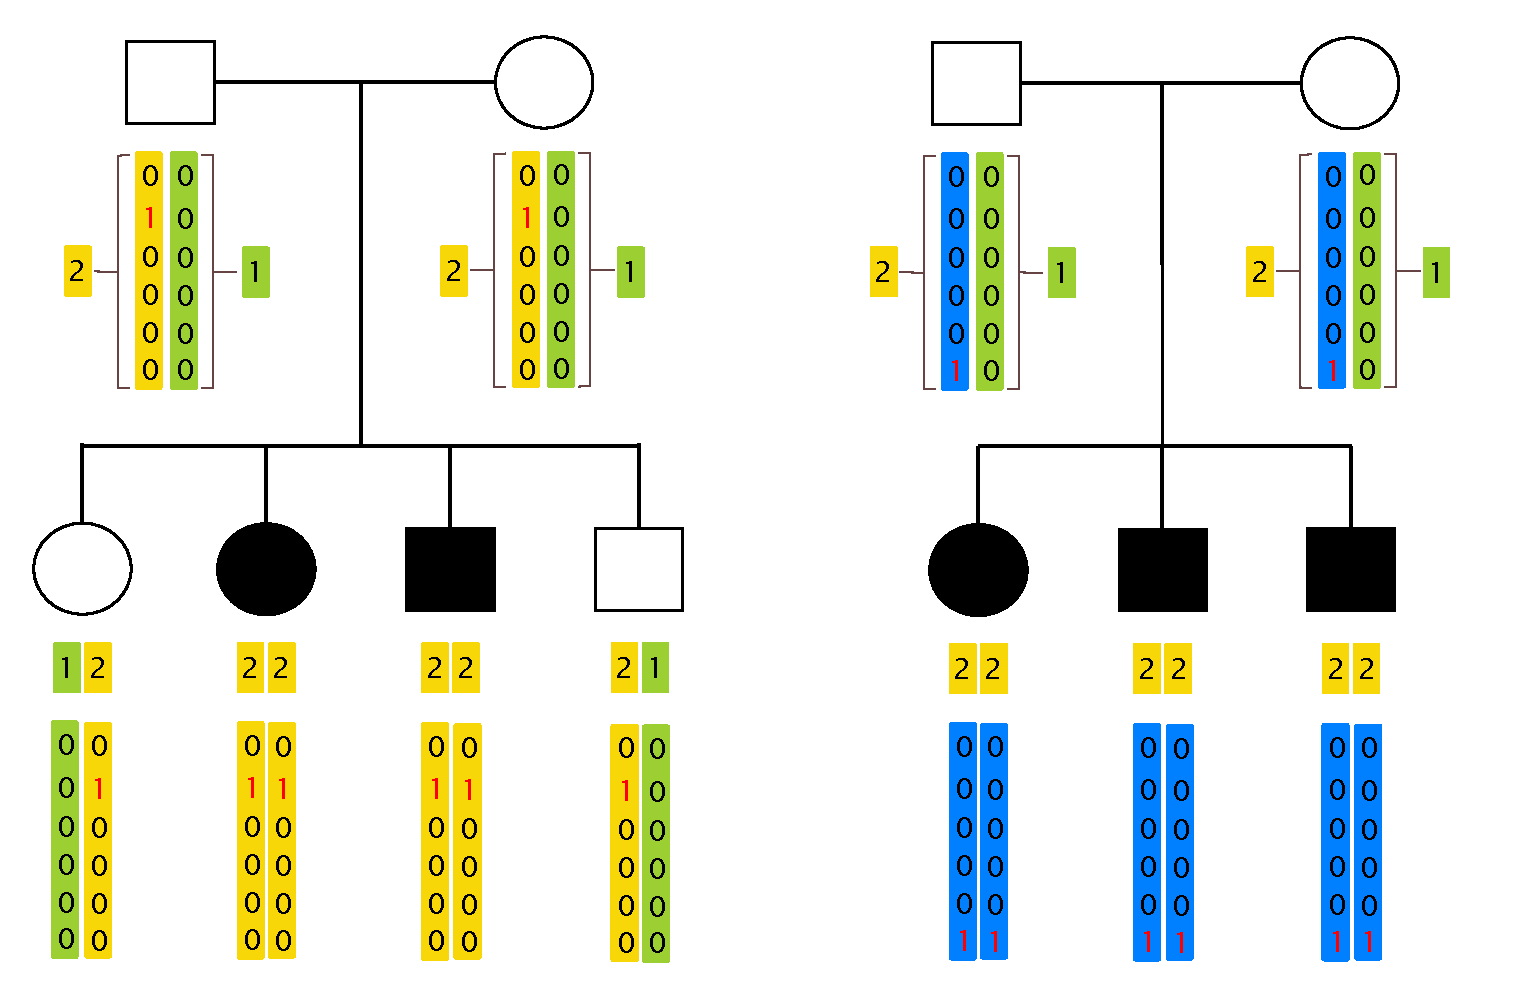
\includegraphics[width=1.0\linewidth]{FigurePresent1.pdf}}
      \end{tabular}
    \end{center} 
    \textbf{\textit{Complete vs. No Collapsing}} 
    \begin{center}
      \begin{tabular}{c}
        \hspace{1em}\scalebox{0.9}{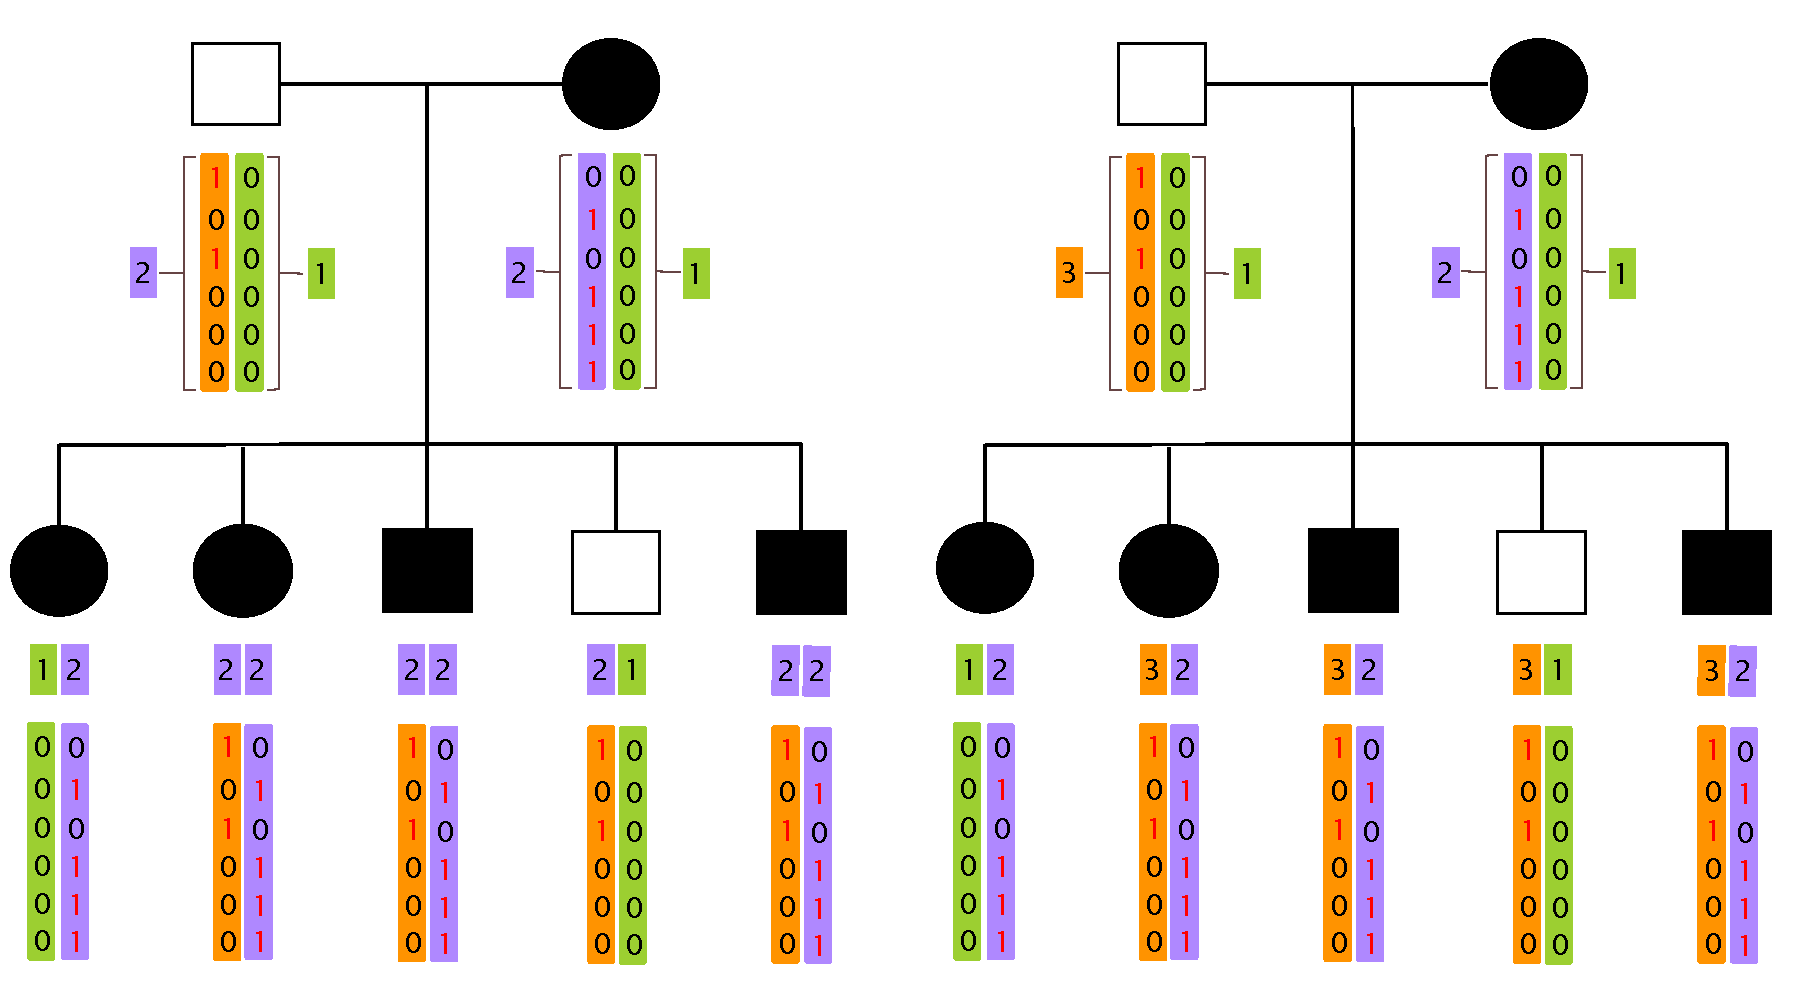
\includegraphics[width=1.0\linewidth]{FigurePresent2.pdf}}
      \end{tabular}
    \end{center} 
  }

%%%%%%%%%%%%%%%%%%%%%%%%%%%%%%%%%%%%%%%%%%%%%%%%%%%%%%%%%%%%%%%%%%%%%%%%%%%%%%
\headerbox{Implementation}{name=covar,column=0,below=stats,above=bottom}{
%%%%%%%%%%%%%%%%%%%%%%%%%%%%%%%%%%%%%%%%%%%%%%%%%%%%%%%%%%%%%%%%%%%%%%%%%%%%%%
    \textbf{\textit{1. Family NGS data preprocessing}}
    \vspace{-0.65em}
    \clist{
        \item[\cir{100}] Mendelian inconsistency check
        \item[\cir{100}] Haplotype reconstruction via genetic phasing 
    }
    \textbf{\textit{2. Regional marker construction}}
    \vspace{-0.65em}
    \clist{
        \item[\cir{100}] Complete collapsing and LD based collapsing themes
        \item[\cir{100}] Sub-regional markers by recombination events 
    }
    
    \textbf{\textit{3. Annotation and statistics for linkage analysis}}
    \vspace{-0.65em}
    \clist{
        \item[\cir{100}] Genetic distance interpolation via \textsl{Rutgers Map}
        \item[\cir{100}] Calculation of marker allele frequencies for linkage analysis with samples having no genotype data 
    }
    \textbf{\textit{4. Parametric test for linkage using regional markers}}
    \vspace{-0.65em}
    \clist{
        \item[\cir{100}] LOD/HLOD scores computed over multiple pedigrees
    }

}

%%%%%%%%%%%%%%%%%%%%%%%%%%%%%%%%%%%%%%%%%%%%%%%%%%%%%%%%%%%%%%%%%%%%%%%%%%%%%%
%  \headerbox{Acknowledgements}{name=ack,column=0,below=analytic,above=bottom}{
%%%%%%%%%%%%%%%%%%%%%%%%%%%%%%%%%%%%%%%%%%%%%%%%%%%%%%%%%%%%%%%%%%%%%%%%%%%%%%
%  \smaller 
%  Many thanks to Dajiang Liu (Leal Lab) and Biao Li (Rice University) for useful discussions and warm support.
%  }%
%%%%%%%%%%%%%%%%%%%%%%%%%%%%%%%%%%%%%%%%%%%%%%%%%%%%%%%%%%%%%%%%%%%%%%%%%%%%%%
  \headerbox{Power analyses and sample size estimations}{name=pow,column=1,span=2}{
%%%%%%%%%%%%%%%%%%%%%%%%%%%%%%%%%%%%%%%%%%%%%%%%%%%%%%%%%%%%%%%%%%%%%%%%%%%%%%
\textbf{\textit{Simulation study design for power analyses}}\\\\\hf{4 nonsyndromic hearing impairment gene sequences} simulated, using sequences from European American samples in NHLBI Exome Sequencing Project; causal variants determined by NCBI-Clinvar database; \hf{two-generational pedigrees} generated with 3 to 8 offspring based on USA population demographic data; \hf{full-penetrance} for causal variants, allowing for \hf{allelic heterogeneity} and varying degrees of \hf{locus heterogeneity}; two-point linkage analysis performed comparing \hf{CHP vs. single variant linkage} methods; empirical power evaluated via 500 replicates\\\\
\textbf{\textit{Power comparisons}}\\\\CHP (orange curves) outperforms single variant linkage method (blue curves) under both dominant (A) and compound recessive (B) models. With 50\% locus heterogeneity it requires \hf{12 families} for CHP to achieve a power of 90\% for \textsl{SLC26A4} at a genome-wide $\alpha$ level of 0.05, while single variant linkage method requires over \hf{50 families}
\begin{center}
  \begin{tabular}{cc}
    \hspace{1em}\scalebox{0.95}{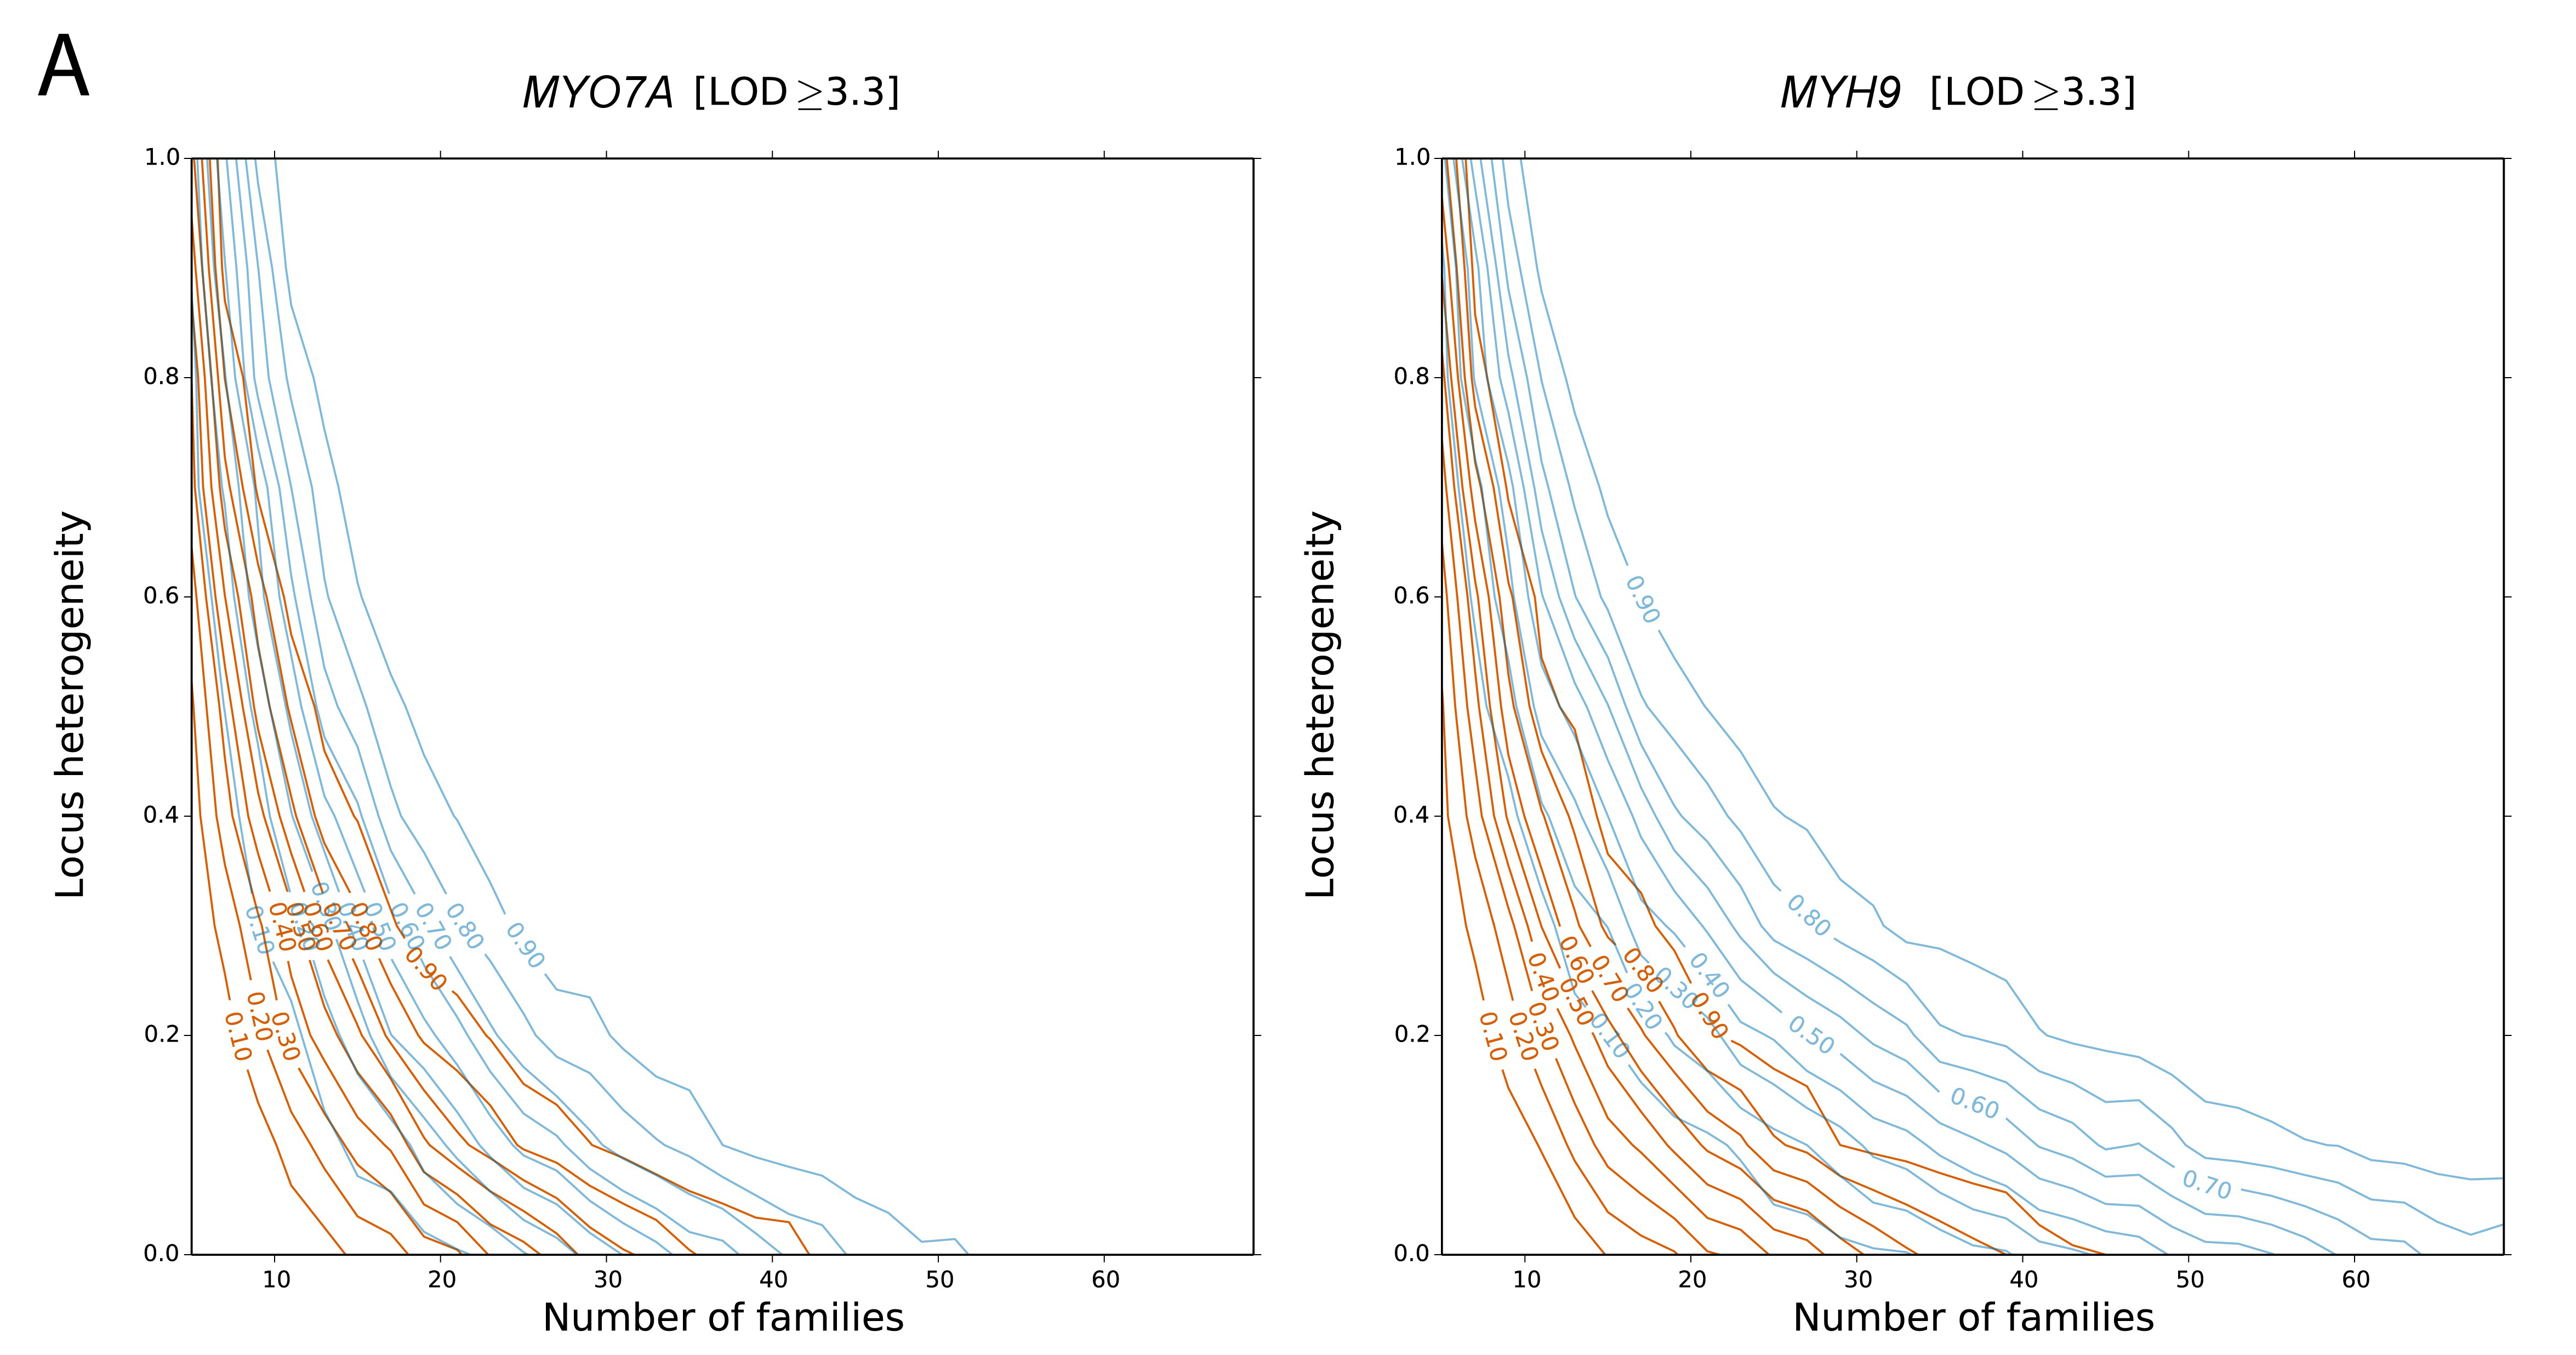
\includegraphics[width=0.5\linewidth]{dom}} &
    \hspace{1em}\scalebox{0.95}{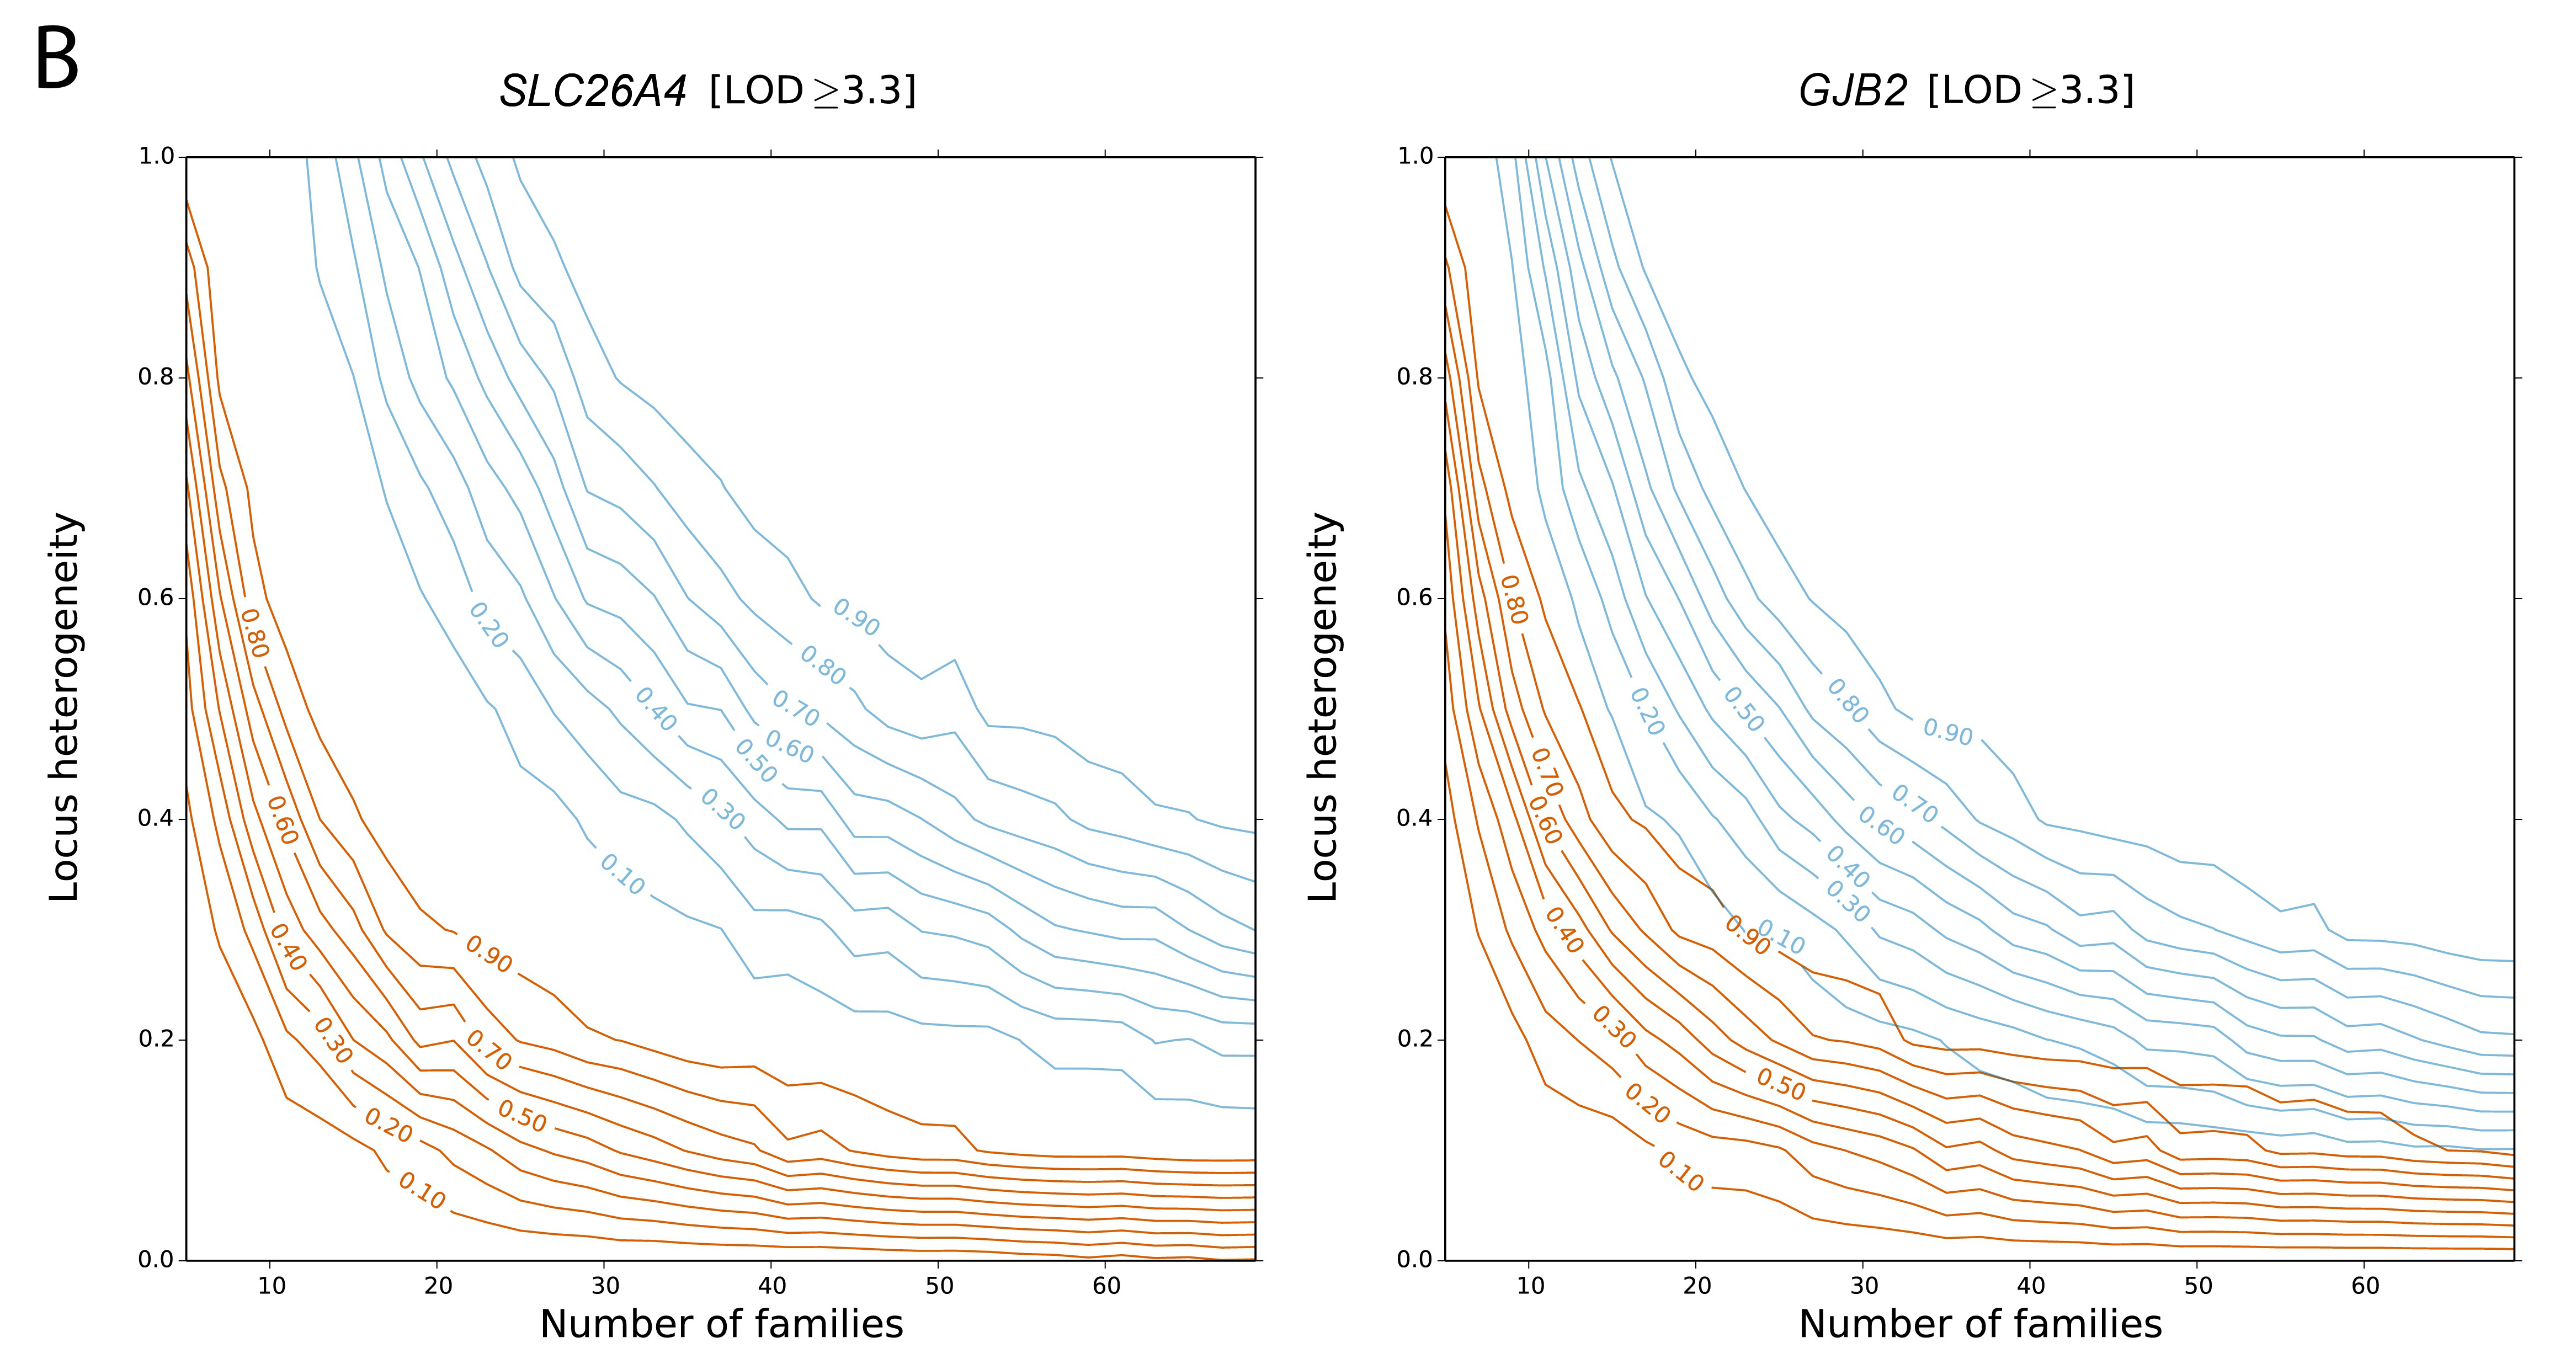
\includegraphics[width=0.5\linewidth]{res}}  
  \end{tabular}
\end{center}
\textbf{\textit{Sample size estimations}}\\\\\hf{Number of families required} to achieve desired power are evaluated; \hf{50\% locus heterogeneity} is assumed for all scenarios; power calculations are based on HLOD score instead; impact of \hf{missing causal variant} in families is evaluated
\begin{center}
{\small \begin{longtable}{ccccccc}
\hline
\textbf{Required Power}&\textbf{Gene}&\textbf{MOI}&\textbf{CHP}$^a$&\textbf{SNV}$^b$&\textbf{CHP-M75}\%$^c$&\textbf{SNV-M75}\%\\
\hline
0.8&\textsl{SLC26A4}&recessive&11&40&39&160\\
0.9&\textsl{SLC26A4}&recessive&13&45&46&180\\
0.8&\textsl{SLC26A4}&compound recessive&11&50&39&200\\
0.9&\textsl{SLC26A4}&compound recessive&13&55&46&220\\
0.8&\textsl{GJB2}&recessive&12&23&44&92\\
0.9&\textsl{GJB2}&recessive&14&28&52&112\\
0.8&\textsl{GJB2}&compound recessive&12&25&44&100\\
0.9&\textsl{GJB2}&compound recessive&14&34&52&136\\
0.8&\textsl{MYO7A}&dominant&12&16&31&64\\
0.9&\textsl{MYO7A}&dominant&14&20&36&80\\
0.8&\textsl{MYH9}&dominant&11&13&32&52\\
0.9&\textsl{MYH9}&dominant&14&18&41&72\\
\hline
\end{longtable}}
\vspace{-0.5em}
{\small a. minimum number of families required to achieve desired power for CHP method}\\
{\small b. minimum number of families required to achieve desired power for single variant linkage method}\\
{\small c. ``M75\%'': minimum number of families requirement when the causal variant in 75\% families are missing}
\end{center}
%% t=`cat SLC26A4.tsv | awk '{if ($3<0.01) sum += $3} END {print sum}'`
%%foo(p, t, x) return(x / (p*t+1-p))
}
%%%%%%%%%%%%%%%%%%%%%%%%%%%%%%%%%%%%%%%%%%%%%%%%%%%%%%%%%%%%%%%%%%%%%%%%%%%%%%
  \headerbox{The SEQLinkage software}{name=imp,column=1,span=1,below=pow}{
%%%%%%%%%%%%%%%%%%%%%%%%%%%%%%%%%%%%%%%%%%%%%%%%%%%%%%%%%%%%%%%%%%%%%%%%%%%%%%
%% \hf{\textit{variant association tools}} is implemented on the backbone of \hf{\textit{variant tools}}. Features include: 
    \clist{
      \item[\cir{100}] Written in \texttt{C++} with a \texttt{Python} parallel computing interface to rapidly scan through markers genome-wide
      \item[\cir{100}] Implements the CHP method for linkage analysis with sequence data of pedigrees in VCF format
      \item[\cir{100}] Supports output of CHP coded markers to formats compatible with other linkage programs
             \clist{
              \item[\tri] \textit{FASTLINK, MEGA2, Merlin, PLINK}
              }
      \item[\cir{100}] Performs two-point linkage analysis involving multiple families, maximizing linkage signals across families to allow for locus heterogeneity (HLOD score calculation)
      \item[\cir{100}] Provides results in text, graphical and table format output, organized with a user-friendly webpage interface
      \item[\cir{100}] Can be used in conjunction with variant filtering method to analyze sequence data of human pedigrees
    }
  SEQLinkage is freely available at
  \begin{center}
  \texttt{http://bioinformatics.org/seqlink} 
  \end{center}
  }
%%%%%%%%%%%%%%%%%%%%%%%%%%%%%%%%%%%%%%%%%%%%%%%%%%%%%%%%%%%%%%%%%%%%%%%%%%%%%%
  \headerbox{Acknowledgments}{name=akc,column=1,span=1,below=imp,above=bottom}{
%%%%%%%%%%%%%%%%%%%%%%%%%%%%%%%%%%%%%%%%%%%%%%%%%%%%%%%%%%%%%%%%%%%%%%%%%%%%%%
    %% \smaller
    %% \vspace{-0.4em}
    %% \renewcommand{\section}[2]{\vskip 0.05em} % removes "References" heading
    %%   \begin{thebibliography}{1}\itemsep=-0.01em
    %%   \setlength{\baselineskip}{0.4em}
    %%   \bibitem{}
    %%     F. Anthony San Lucas, Gao Wang, Paul Scheet, and Bo Peng (2012)
    %%     \newblock Integrated annotation and analysis of genetic variants from next-generation sequencing studies with variant tools
    %%     \newblock In {\em Bioinformatics 28 (3): 421-422.}
    %% \end{thebibliography}

    \vspace{0.4em}
    We would like to thank Regie Lyn Santos-Cortez, Daniel Weeks, Alejandro Schaffer, Jeffrey O'Connell and J\"urg Ott for helpful discussions and support. This work was funded by National Institute of Health grants DC003594, DC011651 and HG006493.
  }%
%%%%%%%%%%%%%%%%%%%%%%%%%%%%%%%%%%%%%%%%%%%%%%%%%%%%%%%%%%%%%%%%%%%%%%%%%%%%%%
  \headerbox{SEQLinkage analysis output}{name=res,column=2,below=pow,above=bottom}{
%%%%%%%%%%%%%%%%%%%%%%%%%%%%%%%%%%%%%%%%%%%%%%%%%%%%%%%%%%%%%%%%%%%%%%%%%%%%%%
    Whole exome sequences of 2 nuclear families each with 4 offspring (3 affected) are analyzed using \hf{SEQLinkage}
    \begin{center}
      \begin{tabular}{c}
        \hspace{1em}\scalebox{0.9}{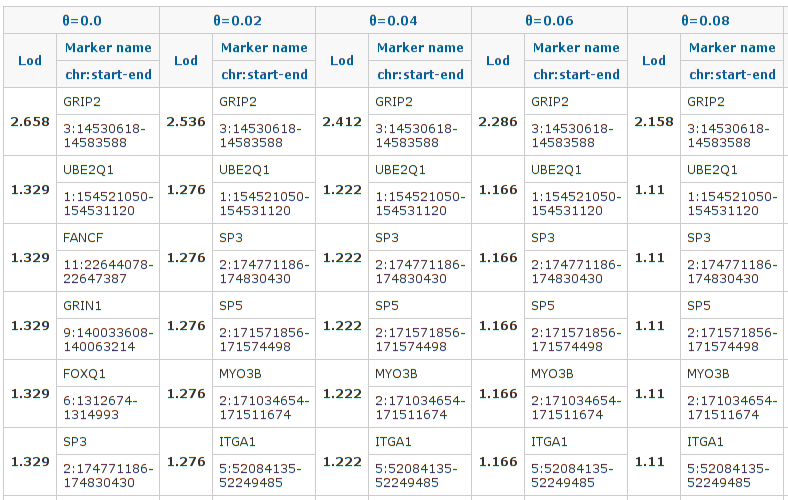
\includegraphics[width=0.8\linewidth]{scrot}}
      \end{tabular}
    \end{center} 
    \vspace{0.2em}
    \begin{center}
      \begin{tabular}{c}
        \hspace{1em}\scalebox{0.9}{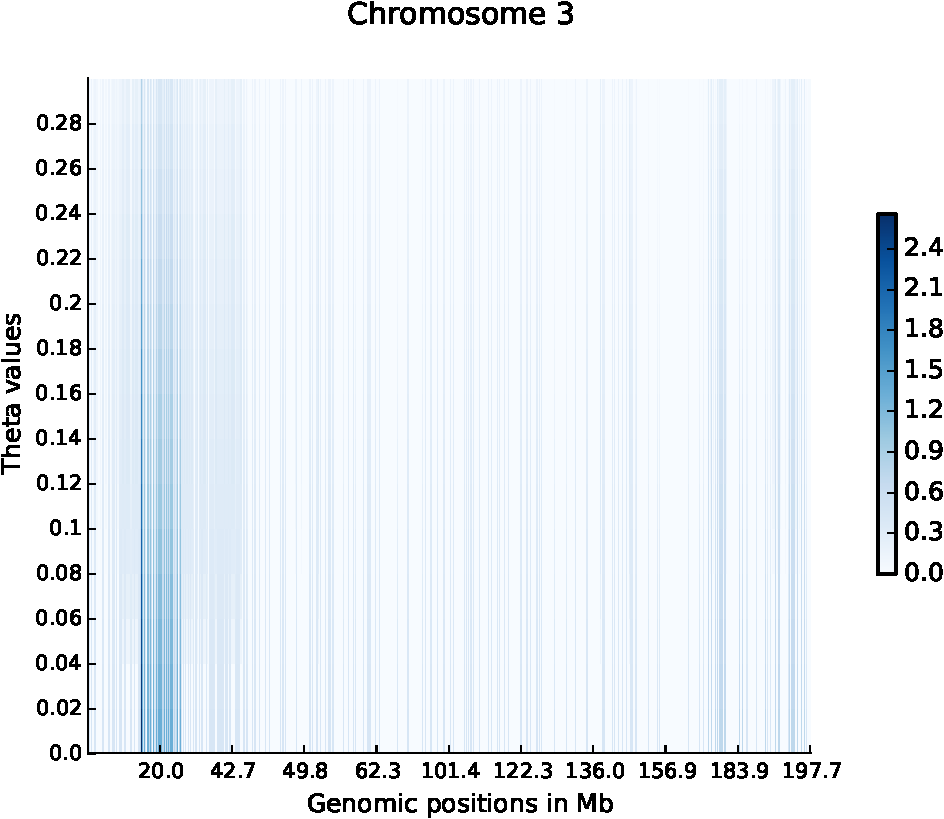
\includegraphics[width=0.8\linewidth]{chr3}}
      \end{tabular}
    \end{center} 
}
\end{poster}%
%
\end{document}
